\section{Voltage Supplies}\label{sec:voltage-supplies}

	\subsection{Power Supplies}\label{ssec:power-supplies}
		In order to avoid any interference of the AC line, this project will work with a DC voltage input and any other necessary voltages will be acquainted from this higher input voltage supply.There are many different types of voltage regulators, nowadays the most common DC/DC being switching regulators. They are more efficient than linear regulators and consequently they waste less heat, the downside is the cost (due their consequently) and that they tend to have some ripple at the output \cite{schweber2017}. However, as this project does not aim radical cost management and as this ripple can be filtered, this type of voltage regulator was choosen for this project.

		\subsubsection{5V Supply}\label{sssec:5v-supply}
			Most of the choosen components for this project were choosen so they would be capable to work with single-supply of 5V. The choosen voltage regulator for the 5V supply was the TL2575-05 from \textit{Texas Instruments} \cite{tl2575-05-datasheet}, it has a output up to 1A, voltage drop ov 2V and typical efficiency of 88$\%$. Figure \ref{fig:tl2575-05-circuit} shows the circuit used for the 5V supply.

			\begin{figure}[htbp]
				\centering
					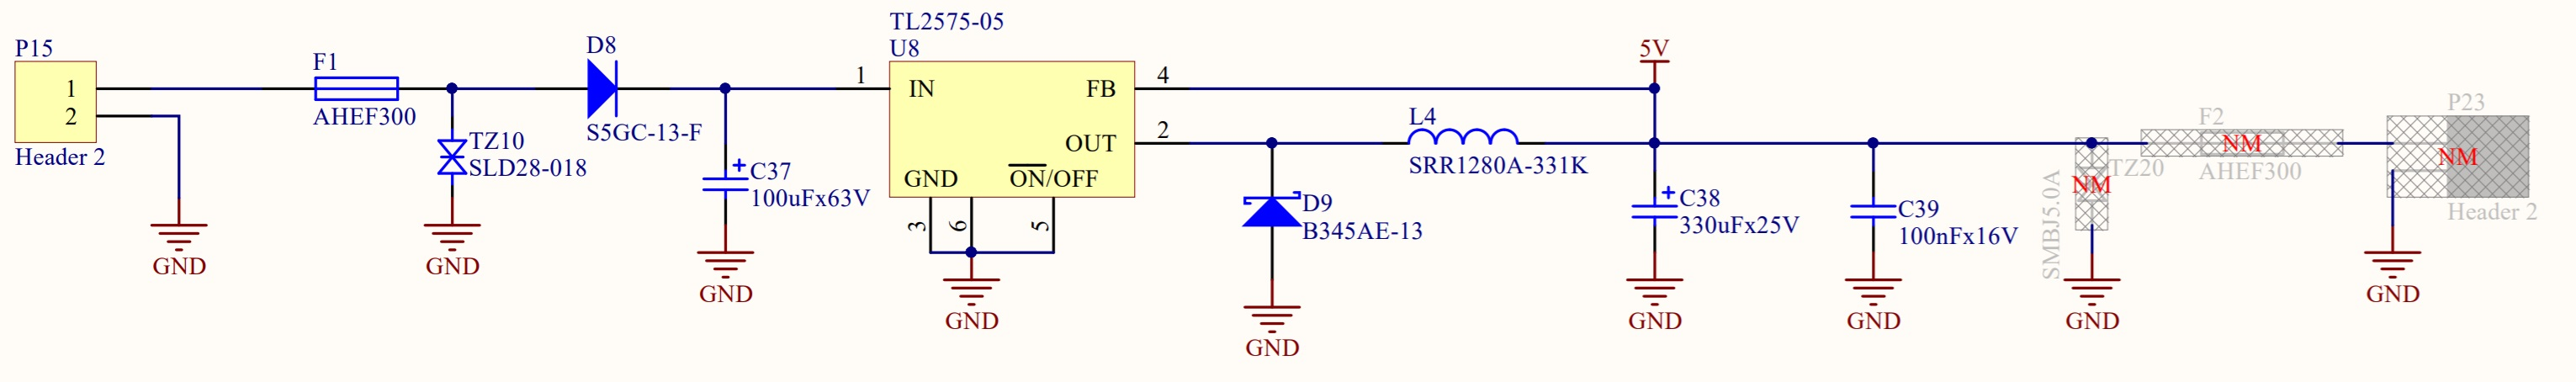
\includegraphics[scale=0.4]{figuras/fig-tl2575-05-circuit.png}
				\caption{5V Power Supply Circuit \cite{tl2575-05-circuit}}
				\label{fig:tl2575-05-circuit}
			\end{figure}

			The diode FM205-W from \textit{Rectron Semiconductor} \cite{fm205-2-datasheet} is used to protect the input of converter from inverse polarity. This diode has a maximum current of 2A, twice the maximum curret output of the regulator, so it will not interfere with the input current. Inductor L4 is fundamental for the device to work according to the datasheet. Capacitors C16 and C17 are a bypass capacitors recommended by the converter's datasheet. Diode D3 is a catch diode used to protect the converter from flyback currents from the inductor, the datasheet only specifies it should be a Schottky diode with maximum current at least the same as the maximum output current of the converter (1A). The choosen diode is FM5819-W from \textit{Rectron Semiconductor} \cite{fm5819-w-datasheet}.
			\par
			According to the datasheet this circuit has a input voltage from 7V to 40V.

		\subsubsection{12V Supply}\label{sssec:12v-supply}
			For the 12V supply the choosen regulator was LM2574-12 from \textit{Texas Instruments} \cite{lm2574-12-datasheet}, it has a output up to 500mA, voltage drop of 2V, and typical efficiency of $88\%$. Figure \ref{fig:lm2574-12-circuit} shows the circuit used for the 12V supply.

			\begin{figure}[htbp]
				\centering
					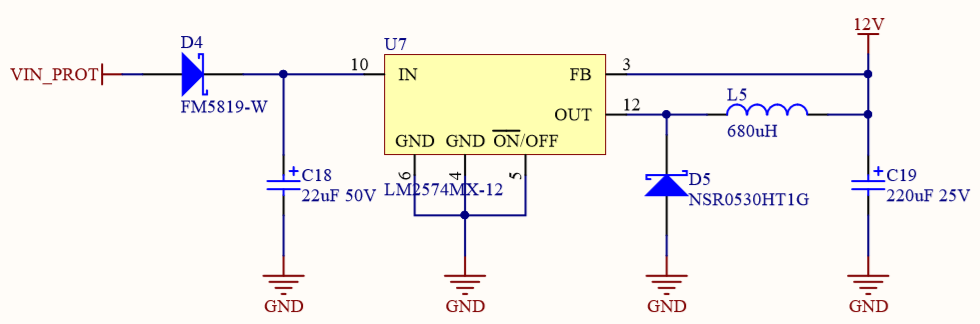
\includegraphics[scale=0.4]{figuras/fig-lm2574-12-circuit.png}
				\caption{5V Power Supply Circuit\cite{lm2574-12-circuit}}
				\label{fig:lm2574-12-circuit}
			\end{figure}	

			The diode FM5819-W from \textit{Rectron Semiconductor} \cite{fm5819-w-datasheet} is used to protect the input of converter from inverse polarity. This diode has a maximum current of 1A, twice the maximum curret output of the regulator, so it will not interfere with the input current. Inductor L5 is fundamental for the device to work according to the datasheet. Capacitors C18 and C19 are a bypass capacitors recommended by the converter's datasheet. Diode D5 is a catch diode used to protect the converter from flyback currents from the inductor, the datasheet only specifies it should be a Schottky diode with maximum current at least the same as the maximum output current of the converter (0.5A). The choosen diode is NSR0530HT1G from \textit{ON Semiconductor} \cite{NSR0530HT1G-datasheet}.
			\par
			According to the datasheet, this circuit has a input voltage from 14V to 40V.	

		\subsubsection{Voltage Input Protection}\label{sssec:voltage-input-protection}

			The voltage that goes to each of the switching voltage regulatores from Sections \ref{sssec:12v-supply} and \ref{sssec:5v-supply} is only protected against inverse polarity but not to overvoltage and overcurrent. Figure \ref{fig:input-protection-circuit} show the circuit used to protect the power supplies.

			\begin{figure}[htbp]
				\centering
					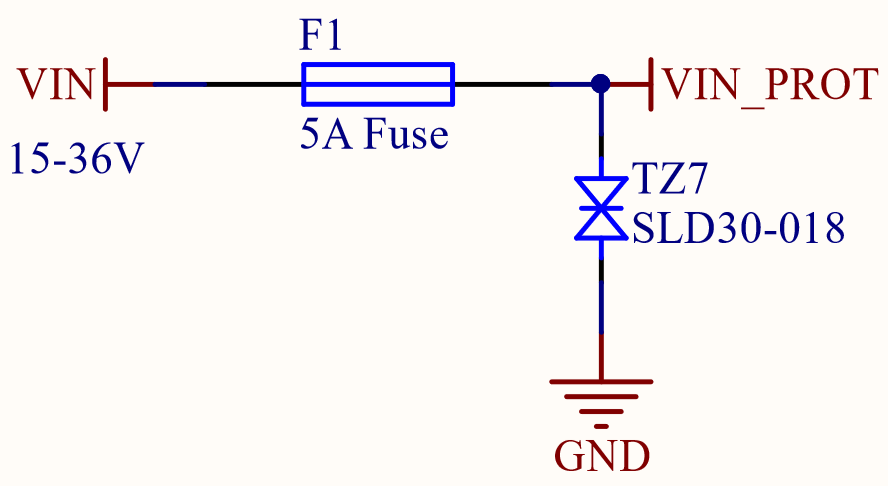
\includegraphics[scale=0.4]{figuras/fig-input-protection-circuit.png}
				\caption{Voltage Input Protection Circuit \cite{input-protection-circuit}}
				\label{fig:input-protection-circuit}
			\end{figure}

			TZ7 is a TVS diode used to protect the circuit against overvoltages. The choosen TVS is the SLD24-018, it has a standoff voltage of 24V and a maximum clamping voltage of 38.9 volts (check Section \ref{ssssec:tvsSelection}). Using this TVS limits the input voltage from 14-24V, in the other hand it ensures protection for the voltage regulators. F1 is a fuse with 5A rating, it will not protect the circuit from fast transients, this will be carried out by the TVS. It has the function to open the circuit when the TVS reaches its clamping voltage and protect the TVS.

	\subsection{Voltage References}\label{ssec:voltage-references}

		In this project any power supply that the precision and stability of the output voltage is more concerning than the maximum output current will be called a voltage reference.

		\subsubsection{10V Reference}\label{sssec:10v-reference}
			As it was explained in Section \ref{ssec:load-cell-signal-conditioning}, this voltage reference will be used to excite the load cells sensors of this project.
		\subsubsection{5V Reference}\label{sssec:5v-reference}
			This reference will be used by the MCU ADC, as said in Item \ref{itm:mcu-aref} from Section \ref{sssec:mcu-power-ports}, a ADC is only as good as it voltage reference. The choosen component for this reference was the LM4040DYM3-5.0-TR from \textit{Microchip} \cite{LM4040DYM3-5.0-TR-datasheet}. According to the datasheet, this voltage reference has a maximum tolerance of $\pm 58mV$ and has maximum operating output current of 15mA. Figure \ref{fig:LM4040DYM3-5.0-TR-circuit} shows to reference circuit.

			\begin{figure}[htbp]
				\centering
					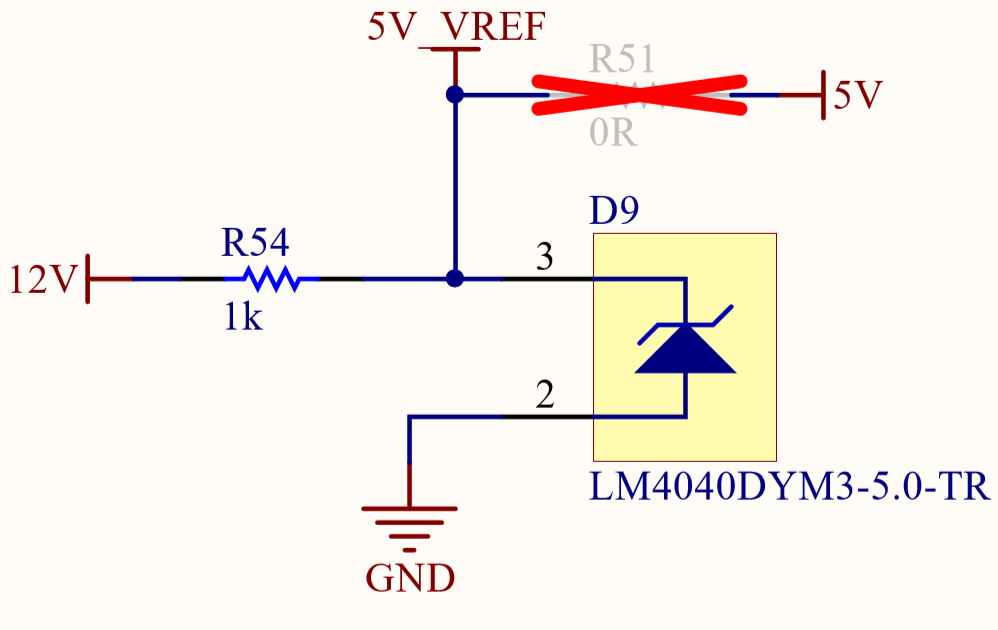
\includegraphics[scale=0.4]{figuras/fig-LM4040DYM3-5.0-TR-circuit.png}
				\caption{10V voltage reference circuit \cite{LM4040DYM3-5.0-TR-circuit}}
				\label{fig:LM4040DYM3-5.0-TR-circuit}
			\end{figure}

			The only external component needed

		\subsubsection{4V5 Reference}\label{sssec:4v5-reference}
		\subsubsection{1V Reference}\label{sssec:1v-reference}